%
\documentclass[11pt]{thesis} % draft

\title{Algorithmic Meta-Creativity}
\author{Fania Raczinski}
\date{March 2015}


\begin{document}


\todo{talk about motivations for using certain things a certain way. I used french text in faustroll because i thought it would be fun.}

\todo{reflect any changes here to the introduction section...}

This project combines research in science, art and the humanities---making it transdisciplinary.

\begin{description}[leftmargin=3cm]
  \item [Pataphysics] Literature, Philosophy, Art
  \item [Creativity] Cognitive Science, \ac{AI}, \ac{DH}
  \item [Technology] \ac{IR}, \ac{NLP}, Web Development
\end{description}

Traditional methodologies in these disciplines are very subject specific and a project combining elements of each field is left mixing and matching suitable methods from them all.

In this chapter I will outline the reasons why none of the existing methodologies are suitable for this project and then explain the choice of more transdisciplinary methods and how I combined them to suit my needs.

\todo{go over intro again when rest is written}

As mentioned in the~\nameref{ch:introduction}\marginnote{§~\ref{s:intromethod}} the overall objectives of this project are to create:

\label{s:objectives}
\begin{enumerate}
  \item three pataphysical search algorithms,
  \item a creative exploratory search tool incorporating the algorithms,
  \item a set of subjective parameters for defining creativity,
  \item an objective framework for evaluating creativity.
\end{enumerate}

Research methods that support these tasks are needed and I will address these four points again at the end of this chapter\marginnote{§~\ref{s:mymeth}}.


\section{Intradisciplinary}

Different disciplines prefer different research methodologies. Of the various disciplines that inform this research the specific subareas that are relevant are as follows.

\begin{itemize}
  \item Information Retrieval
  \item Interface Design
  \item Web Development
  \item Poetry, Literature, and Art
  \item Philosophy
  \item Human and Machine Creativity
  \item Creative Computing
  \item Computational Creativity
\end{itemize}


\subsection{Technology}

Half of this project's objectives are related to computer science therefore it is important to consider how research in this discipline is traditionally approached.

A framework for finding a suitable approach was suggested by Holz et al \citeyear{Holz2006}. The following four steps form an iterative process. ``What do we want to achieve?'' e.g. find out what is happening, develop something that works, evaluate an existing system/technology, compare existing systems, change human behaviour. ``Where does the data come from?'' e.g. how to collect? (read, observe, ask, measure, experiment, model) and where to collect? (field, laboratory, conceptual). ``What do we do with the data?'', e.g. identify themes/patterns/quotes, calculate numbers, identify trends, express via multimedia, create frameworks/taxonomies. ``Have we achieved our goal?'' e.g. draw conclusions, evaluate results, identify limitations.

Another option is to look at what computer science researchers have done historically. In a rather old but still insightful analysis of over \num{600} papers\footnote{While the paper itself was published in 2004, the body of work they studied was based on publications from between 1995 and 1999---this suggests that a lot of the more ``recent'' research around Web technologies is not included in this study.} Ramesh et al \citeyear{Ramesh2004} have shown that---by far---the most common approach to research in computer science during this period was \emph{formulative} with almost 79\% use (as opposed to ``descriptive'' with 10\% and ``evaluative'' with 11\%) in particular in regards to ``processes, methods and algorithms'' which was used by just over 50\% of researchers. Not surprisingly the most popular research method was \emph{mathematical conceptual analysis} with about 75\% use.

Jose Nelson Amaral \citeyear{Amaral} classifies methodologies in computer science into five main categories as shown below.

\begin{description}[leftmargin=3.5cm]
  \item [Formal] Proof, verification, correctness
  \item [Experimental] Testing, evaluation, question answering
  \item [Build] Proof of concept, prototype, artefact
  \item [Process] Understand and define processes
  \item [Model] Abstraction, simulations
\end{description}

\spirals

Based on \autocite{Holz2006}, here are this projects answers to the four questions posed in the research.

\begin{description}
  \item[What do we want to achieve?]~
    - Understand human creativity and how this translates to machines.\\
    - Understand the relationship of pataphysics and creativity.\\
    - Understand how creativity is evaluated in humans and machines.\\
    - Research suitable pataphysical concepts to be implemented as algorithms.\\ 
    - Define algorithms formally.\\
    - Implement prototype incorporating algorithms.\\
    - Develop framework for interpreting and evaluating machine creativity.
	\item[Where does the data come from?]~
    - Read pataphysical literature and research.\\
    - Collate existing research on creativity and evaluation.\\
    - Survey creative approaches to technology.\\
    - Experimentation with algorithms and implementation.
	\item[What do we do with the data?]~
    - Iterate through developmental stages of algorithmic outputs.\\
    - Create an artefact that represents the underlying philosophy and research as a whole.\\
    - Create evaluation framework based on theoretical research.
  \item[Have we achieved our goal?]~
    - See conclusion chapter~\ref{ch:observations}\marginnote{§~\ref{ch:observations}}.
\end{description}

Referring back to the objectives above (see page~\pageref{s:objectives}), objective \num{1} is to create new creative search algorithms. This is not supposed to happen on a purely abstract basis but in a practical fashion (`experimental'), with a working implementation (`build') as proof of concept (see objective 2). While the algorithms need to be defined in formal terms (`formal'), the goal here is not to create a theoretical proof of correctness (given the creative and rather subjective nature of the underlying philosophy this is virtually impossible) but a practical demonstration of the creative processes behind. Given the creative nature of the algorithms, rigorous testing would be irrelevant. Overall this would suggest an experimental approach with prototyping of an artefact. Objective \num{3} is to come up with a suitable definition of creativity (`process'). This should be informed by existing research. Again, we are not interested in formulating this in mathematical terms and proofs but rather a more esoteric and systemic view. Because the definition needs to apply to humans and machines it needs to be precise enough. Objective \num{4} is then to create an overall theoretical framework (`model') for the evaluation of creativity in humans and machines.

By now we have managed to cover every one of the major methodologies mentioned in \autocite{Amaral} but we are still lacking ways to address the subjective and creative nature of the project. Furthermore, the philosophical and artistic inspirations that inform the development of the artefact don't get enough of a voice in these methods. In computer science, implementations are generally seen as a proof of concepts or prototypes---when really they should be seen as artefacts in the sense of artistic pieces of work. So, to really appreciate the scope of this practical element of this project we need to consider research in the arts and humanities too.


\subsection{Arts and Humanities}

% \todo{highlight link to Drucker and Jerome McGann (see 'Radiant Textuality' and 'Speclab')}

\begin{quotation}
  A hallmark of humanistic study is that research is approached differently than in the natural and social sciences, where data and hard evidence are required to draw conclusions. Because the human experience cannot be adequately captured by facts and figures alone, humanities research employs methods that are historical, interpretive and analytical in nature. \sourceatright{\autocite{Standford2016}}
\end{quotation}

Malins and Gray suggest the following ideas for arts-based researchers searching for the right methodology \citeyear{Malins1995}.

\begin{itemize}
  \item Consider a range of research strategies (from all disciplines)
  \item `Tailor' the research project to the nature of project and the researcher's expertise
  \item Carry out the research from the informed perspective of the reflective practitioner, as `participant observer'
  \item Continually define and refine the research question, allowing methodologies to emerge
  \item Acknowledge accessibility, discipline, rigour, transparency, transferability
  \item Be aware of the critical context of practice and research and raise the level of critical debate
  \item Consider interdisciplinary / multidisciplinary approaches to research
\end{itemize}

They further elaborate on the key characteristics of arts methodologies as follows \autocite{Gray2004}.

\begin{quotation}
\begin{itemize}
  \item Experiencing/exploring, gathering, documenting information and generating data/evidence
  \item Reflecting on and evaluating information, selecting the most relevant information
  \item Analysing, interpreting and making sense of information
  \item Synthesizing and communicating research findings, planning new research
\end{itemize}\sourceatright{\autocite{Gray2004}}
\end{quotation}

They specify a whole set of individual methods used for the approaches above.

\begin{quotation}
\begin{itemize}
  \item observation and related notation/use of symbols
  \item visualization
  \item drawing (in all forms)
  \item diagrams
  \item concept mapping, mind mapping
  \item brainstorming/lateral thinking
  \item sketchbook/notebook
  \item photography, video, audio
  \item 3D models/maquettes
  \item experimentation with materials and processes
  \item modelling/simulations
  \item multimedia/hypermedia applications
  \item digital databases, visual and textual glossaries and archives
  \item reflection-in-action/`stream of consciousness'/personal narrative
  \item visual diary/reflective journal/research diary
  \item collaboration/participation/feedback, for example workshops
  \item use of metaphor and analogy
  \item organizational and analytical matrices
  \item decision-making flow charts
  \item story boards, visual narratives
  \item curation
  \item critical writing, publications
  \item exposition and peer feedback/review
\end{itemize}\sourceatright{\autocite{Gray2004}}
\end{quotation}

The discpiline of \ac{DH} (see chapter~\ref{s:digithuman}\marginnote{§~\ref{s:digithuman}}) seems like a logical choice to look for suitable methodologies. It is characterised by ``collaboration, transdisciplinarity and an engagement with computing'' \autocite{Burdick2012} but it should not simply be reduced to `doing the humanities digitally' \autocite{Burdick2012}. Transliteracy, an understanding of several kinds of tools and media, is an important aspect in this \autocite{Thomas2007}. \ac{DH} can be broken down into the following set of methodologies.

\begin{description}
  \item [Design] shape, scheme, inform, experience, position, narrate,
  					interpret, remap/reframe, reveal, deconstruct, reconstruct,
  					situate, critique
  \item [Curation, analysis, editing, modelling] digitise, classify, describe, metadata, organise, navigate
  \item [Computation, processing] disambiguate, encode, structure, procedure, index, automate, sort, search, calculate, match
  \item [Networks, infrastructure] cultural, institutional, technical, compatible, interoperable, flexible, mutable, extensible
  \item [Versioning, prototyping, failures]	iterate, experiment, take-risks, redefine, beta-test
\end{description}

Some of the emerging methods Burdick et al. have identified are listed below \citeyear{Burdick2012} (The full list can be found in appendix~\ref{s:dhmap}\marginnote{§~\ref{s:dhmap}}).

\begin{itemize}
  \item structured mark-up
  \item	natural language processing
  \item	mutability
  \item	digital cultural record
  \item	algorithmic analysis
  \item distant/close, macro/micro, surface/depth
  \item parametrics
  \item	cultural mash-ups
  \item	algorithm design
  \item data visualization
  \item	modelling knowledge
  \item	ambient data
  \item	collaborative authorship
  \item	interdisciplinary teams
  \item	use as performance
  \item narrative structures
  \item	code as text
  \item	software in a cultural context
  \item repurposable content and remix culture
  \item participatory Web
  \item	read/write/rewrite
  \item	meta-medium
  \item	polymorphous browsing
\end{itemize}

\spirals

Applying the above methodologies from the arts and \ac{DH} to my research is useful. Several of the overall methodologies listed by Gray and Malins \citeyear{Gray2004} seem to apply to the research presented in this thesis. Exploring, evaluating, analysing, interpreting, synthesising and disseminating research all are part of it. However, looking at the specific methods they collated the difference becomes clearer as only the following 7 apply remotely (Visualization, experimentation with processes, multimedia/hypermedia applications, use of metaphor and analogy, organizational and analytical matrices, curation, and critical writing, publications).

The \ac{DH} methodologies seem more useful. In terms of `design', \url{pata.physics.wtf} positions itself in context and the evaluation framework interprets and critiques \ac{AMC}. Before that I `curate' the two corpora, digitise them and organise them. `Computing' comes in at verious stages, to (dis)ambiguate (i.e. pataphysicalise), encode, index, search and match data. The `infrastructure' is cultural, technical and extensible, relying on the \ac{WWW} for several spects. `Versioning, prototyping and failures' all come in during the iterative development process, which involves a lot of experimentation and refactoring. Furthermore, the methods Burdick et al \citeyear{Burdick2012} list match this project much better.


\section{Transdisciplinary}

Basarab Nicolescu distinguished between three different kinds of research `without stable boundaries between the disciplines'.\footnote{Nicolescu cites Jean Piaget here, who first coined the term `transdisciplinarity' in 1972.} \citeyear{Nicolescu2010}.

\begin{description}
  \item [Multidisciplinarity]	concerns itself with studying a research topic in not just one discipline but in several simultaneously.
  \item [Interdisciplinarity]	concerns the transfer of methods from one discipline to another.
  \item [Transdisciplinarity]	concerns that which is at once between the disciplines, across the different disciplines, and beyond all disciplines.
\end{description}

The standard epistemological view of science and art is that they are objective and subjective, respectively. So, what does that mean for research conducted between, across and beyond science and art, i.e. research that is transdisciplinary?

Nicolescu criticises the view that science must be objective. He even claims that any non-scientific knowledge is ``cast into the inferno of subjectivity, tolerated at most as a meaningless embellishment or rejected with contempt as a fantasy, an illusion, a regression, or a product of the imagination'' \citeyear{Nicolescu2010}. Objectivity, he says, becomes the `supreme criterion of Truth'\footnote{As we shall see later, pataphysics does the opposite: it reveres the Subject.}

\begin{quotation}
  The death of the Subject is the price we pay for objective knowledge. \sourceatright{\autocite{Nicolescu2010}}
\end{quotation}

He goes on to quote Werner Heisenberg on the concepts of objective and subjective reality: ``we would make a very crude simplification if we want to divide the world in[to] one objective reality and one subjective reality. Many rigidities of the philosophy of the last centuries are born by this black and white view of the world'' \autocite[Heisenberg, cited in][]{Nicolescu2010}.

\begin{quotation}
  The too strong insistence on the difference between scientific knowledge and artistic knowledge comes from the wrong idea that concepts describe perfectly the `real things'. [\ldots] All true philosophy is situated on the threshold between science and poetry. \sourceatright{\autocite[Heisenberg, cited in]{Nicolescu2010}} \footnote{The full paragraph is worth quoting---see appendix~\ref{s:heisenberg}.}
\end{quotation}

In transdisciplinarity traditional disciplinary boundaries have no meaning.

\begin{figure}[!htbp]
\centering
  \begin{tikzpicture}
    \node [box] at (1.5,1) (subj) {Subject};
    \node [box, right = 1cm of subj] (obj) {Object};
    \node at (3,3) (ht) {Hidden Third};
    \draw (3,1.75) circle [radius=3cm]; 
    \node at (6.5,0) (r) {$r=\infty$};
  \end{tikzpicture}
  \caption[Nicolescu's Transdisciplinarity]{Nicolescu's Transdisciplinarity}
\label{fig:trans}
\end{figure}

Working across disciplines requires a new unique methodology. Nicolescu proposes a methodology of transdisciplinarity as a non-hierarchical ternary partition of `Subject, Object and Hidden Third'\marginnote{\faicon{object-group}~\ref{fig:trans}} rather than the traditional binary partition of `Subject versus Object' \citeyear{Nicolescu2010}.

\begin{quotation}
  The old principle ``unity in diversity and diversity from unity'' is embodied in transdisciplinarity.' \sourceatright{\autocite{Nicolescu2010}}
\end{quotation}

\spirals

This project positions itself ``at once between the disciplines, across the different disciplines, and beyond all disciplines''---making it transdisciplinary. The abolishment of disciplinary boundaries suits the unique context of this research. Pataphysics specifically is highly subjective. John Searle highlighted that ontologically subjective topics (such as creativity) can be studied in epistemically objective ways \citeyear{Searle2015}.

 




\subsection{Hugill and Yang Methodology}

\begin{quotation}
  `unite and conquer' vs `divide and conquer' \sourceatright{\autocite[p.1]{Yang2013}}
\end{quotation}
\todo{rephrase}

\begin{draft}
  Hugill and Yang suggest that existing research methodologies are unsuitable for transdisciplinary subjects such as \ac{CC}. The following is an example of a possible \ac{CC} research methodology they propose as a starting point \autocite[p.17]{Hugill2013c}:

  \begin{enumerate}
    \item Review literature across disciplines
    \item Identify key creative activities
    \item Analyse the processes of creation
    \item Propose approaches to support these activities and processes
    \item Design and implement software following this approach
    \item Experiment with the resulting system and propose framework
  \end{enumerate}

  They go on to propose four standards for \ac{CC} \autocite[p.17]{Hugill2013c} namely, resist standardisation, perpetual novelty, continuous user interaction and combinational, exploratory and or transformational.
\end{draft}

\begin{draft}

\end{draft}

\subsection{Practice Based}

Linda Candy defines practice based research as follows.

\begin{quotation}
  Practice-based Research is an original investigation undertaken in order to gain new knowledge partly by means of practice and the outcomes of that practice. \sourceatright{\autocite{Candy2006}}
\end{quotation}

She further explains that original contributions to knowledge required in PhD projects can be demonstrated through creative outcomes `in the form of designs, music, digital media, performances and exhibitions' \autocite{Candy2006}.

% \begin{fcom}
%   my practice is software development but framed in arty bollocks.
% \end{fcom}

\todo{finish section on practice based research here}

% \begin{quote}
%   ``Art research is of necessity speculative research. It produces its own protocols; the artist as researcher engages with knowledge in ways that involve the adoption of new frames of reference, the design of new systems and the acquisition of new behaviours. Outcomes will be generally non-linear, associative, connective, transformative and frequently challenging. Trans-disciplinary research in art generates discourse requiring new language.''\autocite[Roy Ascott's preface in][p. v]{Candy2011}
% \end{quote}

% \begin{quote}
%   ``In ways often disconcerting to its academic hosts, art research is prepared to look in all directions for inspiration, understanding and explication: to the East as well as the West, so to speak; following the left-hand path as well as the right; working with both reason and intuition, sense and nonsense, subtelty and sensibility. It is what can be called a transdisciplinary syncretism that best informs artistic research, just as it is the integrative faculty of ‘cyberception’ that enables our focus on mutliple realities and a technoetic instrumentality that supports art strategies involving the evolution of mind, the networked distribution of presence and the re-configuration of personal identity. Art research is second-order research; the researcher is always a part of the system or subject of inquiery. Innovation in subjectivity prevails over odurate objectivity. [...] methodologies that can, whenever needed, put subject before object, process before system, behaviour before form, intuition before reason and mind before matter.''\autocite[Roy Ascott's preface in][p. vi]{Candy2011}
% \end{quote}

\begin{figure}[!htbp] % (here, top, bottom, page)
  \centering
  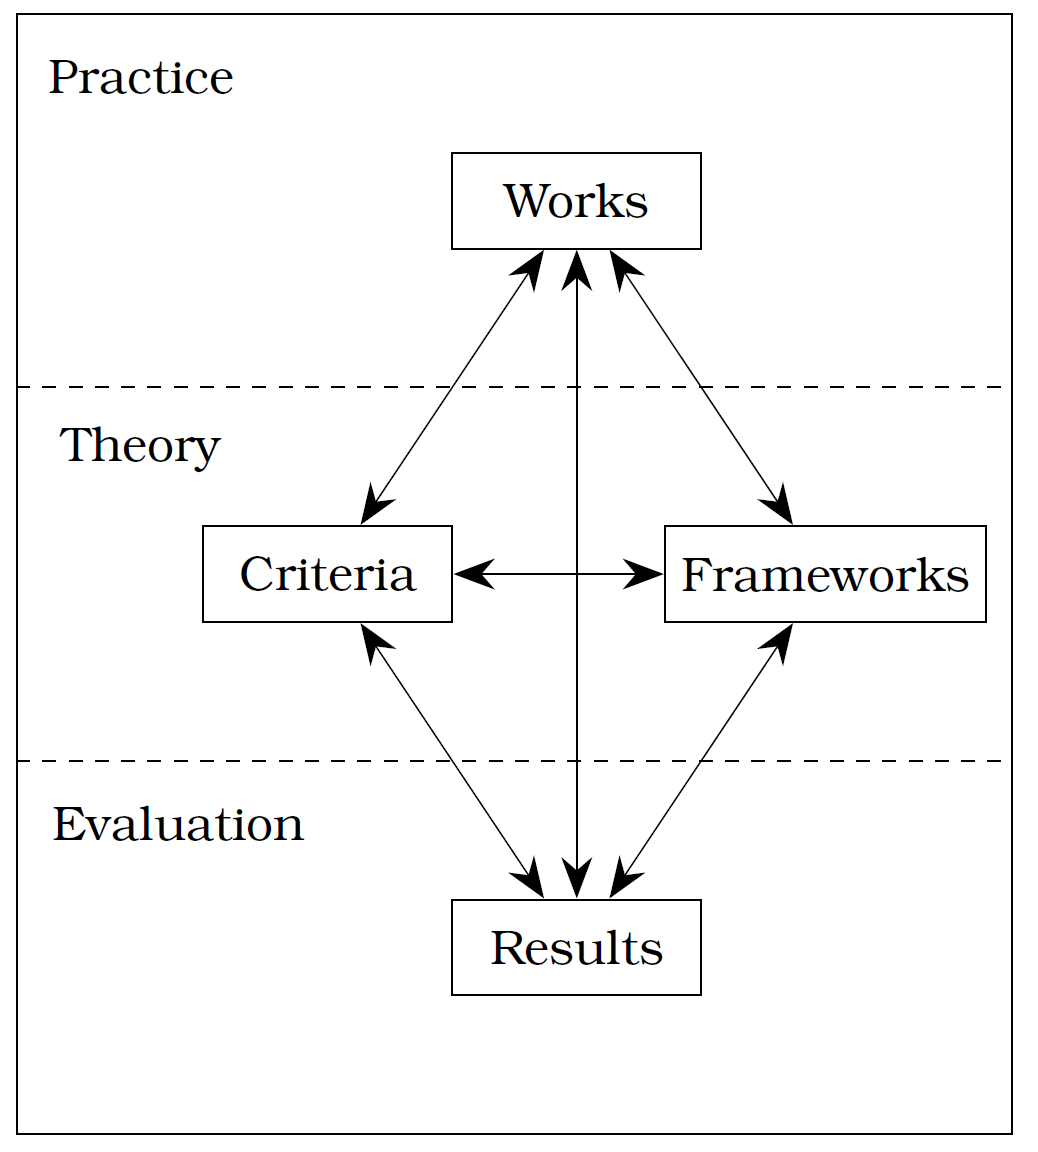
\includegraphics[width=.5\textwidth]{tmpr}
  \caption[Trajectory Model]{Edmonds and Candy's Trajectory Model (W = Works, C = Criteria, F = Frameworks, R = Results)}
\label{fig:tmpr}
\end{figure}

\begin{tikzpicture}
	\draw (0,0) rectangle (8,9);
    \draw [draw,dashed] (0,3) -- (8,3);
    \draw [draw,dashed] (0,6) -- (8,6);
    \node at (1,8.5) (p) {Practice};
    \node at (1,5.5) (t) {Theory};
    \node at (1,2.5) (e) {Evaluation};
%     \node [draw, minimum height = 2em, minimum width = 2em] at (4.5,1.5) (results) {R};
%     \node [draw, minimum height = 2em, minimum width = 2em] at (2.5,4.5) (criteria) {C};
%     \node [draw, minimum height = 2em, minimum width = 2em] at (6.5,4.5) (frameworks) {F};
%     \node [draw, minimum height = 2em, minimum width = 2em] at (4.5,7.5) (works) {W};
    \node [box] at (4.5,1.5) (results) {Results};
    \node [box] at (2.5,4.5) (criteria) {Criteria};
    \node [box] at (6.5,4.5) (frameworks) {Frameworks};
    \node [box] at (4.5,7.5) (works) {Works};
    \draw [<->] (results) -- (criteria);
    \draw [<->] (results) -- (frameworks);
    \draw [<->] (results) -- (works);
    \draw [<->] (works) -- (criteria);
    \draw [<->] (works) -- (frameworks);
    \draw [<->] (criteria) -- (frameworks);
\end{tikzpicture}

Figure~\ref{fig:tmpr}\marginnote{\faicon{object-group}~\ref{fig:tmpr}} shows the \ac{TMPR} developed by Ernest Edmonds and Linda Candy as a framework to `influence practice, inform theory and, in particular, shape evaluation' \autocite{Edmonds2010}. The model allows for different trajectories between practice, theory and evaluation. Table~\ref{tab:tmpr}\marginnote{\faicon{table}~\ref{tab:tmpr}} shows the various elements, activities and outcomes in this framework more clearly.

\begin{table}[!htbp]
\caption[Elements, Activities and Outcomes of the \ac{TMPR}]{Elements, Activities and Outcomes of each Trajectory in the \ac{TMPR}}
\label{tab:tmpr}
  \begin{tabu}{X[1]X[2]X[3]}
  \toprule
  \textbf{Elements}
  &
  \textbf{Activities}
  &
  \textbf{Outcomes}
  \\ \midrule
  \textbf{Practice}
  &
  create, exhibit, reflect
  &
  \textbf{Works:} consisting of physical artefacts, musical compositions, software systems, installations, exhibitions, collaborations
  \\ \midrule
  \textbf{Theory}
  &
  read, think, write, develop
  &
  \textbf{Frameworks:} comprising questions, criteria, issues
  \\ \midrule
  \textbf{Evaluation}
  &
  observe, record, analyse, reflect
  &
  \textbf{Results:} findings leading to new/modified Works and Frameworks
  \\ \bottomrule
  \end{tabu}
\end{table}


\section{My Research Approach}
\label{s:mymeth}

\todo{rapid incremental prototyping}

The doctoral research presented in this thesis does not fit into neat categories in science or art---making it transdisciplinary in nature. Subjects like literature, philosophy, cognitive science, artificial intelligence, software engineering and linguistics frame the three core areas of research for this project, namely pataphysics, creativity and computing.

To address the transdisciplinary nature of the project I 


employed a practice-based research methodology, meaning that part of my submission for the degree of Doctor of Philosophy is an artefact demonstrating my original contribution to knowledge. The thesis provides the context of this artefact and critically analyses and discusses the experimental process and outcome.

\begin{description}
  \item [Epistemology] Transdisciplinary, Subjective
  \item [Methodology] Qualitative, Exploratory
  \item [Methods] Creative Computing, Website Development, Literature Review, Evaluation Framework, Critical Reflection
\end{description}

The general workflow of my project was as follows.
\begin{draft}
relates back to hugill and yang approach
\end{draft}

\begin{enumerate}
  \item Conduct extensive literature review into the various subjects involved,
  \item develop pataphysical algorithms,
  \item develop an evaluation framework,
  \item design a system to demonstrate algorithms,
  \item develop a website for the tool,
  \item evaluate website using framework and redevelop as needed and
  \item write up findings.
\end{enumerate}

In regards to the practice based methodology, I followed the following trajectory inspired by the \ac{TMPR}\marginnote{\faicon{object-group}~\ref{fig:tmpr}}.

\todo{create my own tmpr figure here}

\begin{description}
  \item [Practice] (Works): Implementation of Algorithms, Development of Website
  \item [Theory] (Criteria, Frameworks): Creation of Algorithms, Setting Context, Define Evaluation Framework
  \item [Evaluation] (Results): Interpretation of Work
\end{description}

\begin{draft}
  This tmpr is my thesis.\\
  works: pata.physics.wtf\\
  criteria: criteria for creativity\\
  frameworks: evaluation framework\\
  results: conclusion
\end{draft}

\begin{draft}
  does the tpmr fit into the hugill and yang approach?
\end{draft}



The general process\marginnote{§~\ref{ch:implementation}} of my project was as follows.

\begin{enumerate}
  \item Conduct extensive literature review into the various subjects involved,
  \item develop pataphysical algorithms,
  \item develop an evaluation framework,
  \item design a system to demonstrate algorithms,
  \item develop a website for the tool,
  \item evaluate website using framework and redevelop as needed and
  \item write up findings.
\end{enumerate}


\todo{comp creat vs creat comp}
\begin{draft}
  list out the different examples of why my project is both of the above. 
  eg it is comp creat because i use javascript+maths for display the poetry
  but creat comp is the mis-use of damerau levensthein algorithm
\end{draft}

\end{document}
